% !TEX TS-program = xelatex
\documentclass[10pt, conference]{IEEEtran}
\usepackage{fontspec}
\usepackage{dirtytalk}
\usepackage{tikz}
\usepackage{listings}
\usepackage[cmintegrals]{newtxmath}
\usepackage{bm}
\usepackage{biblatex}
\setmainfont{QTBookmann}
\lstset{basicstyle=\ttfamily\tiny, breaklines=true}
\usetikzlibrary{positioning}
\bibliography{bibliography.bib}
 \tikzset{
   x=2.8em,
   y=2.8em,
 }
%! TeX program = xelatex
%! TeX TS-program = xelatex
%! TeX root = ProgramaciónEvolutiva.tex
%%%%%%%%%%%%%%%%%%%%%%%%%%%%%%%%%%%%%%%%%%%%%%%%%%%%%%%%%%%%%%%%%%%%%%%%
% Define AntiqueWhite color
\definecolor{AntiqueWhite}{RGB}{250,235,215}
\definecolor{mypurple}{RGB}{104,020,108}
\setbeamercolor*{palette primary}{use=structure,fg=white,bg=mypurple}
\setbeamercolor{normal text}{fg=white, bg=black}
\setbeamercolor{tcolorbox text}{fg=white, bg=black}
\setbeamertemplate{navigation symbols}{}                              %
\newcommand{\colouredcircle}{%
  \tikz{\useasboundingbox (-0.2em,-0.32em) rectangle(0.2em,0.32em);
        \draw[ball color=PineGreen!7!Plum!90!Red,shading=ball,line width=0.03em] (0,0) circle(0.18em);}}
\newcommand{\colouredcircledis}{%
  \tikz{\useasboundingbox (-0.2em,-0.32em) rectangle(0.2em,0.32em);
        \draw[ball color=PineGreen!7!Plum!20!Black,shading=ball,line width=0.03em] (0,0) circle(0.18em);}}
\setbeamertemplate{itemize item}{\colouredcircle}
\setbeamercolor*{bibliography entry title}{fg=Yellow!80!White, bg=Black}
% Set beamer bibliography titles and numbers color to antique white
\setbeamercolor*{bibliography entry author}{fg=AntiqueWhite}
\setbeamercolor*{bibliography entry location}{fg=AntiqueWhite}
\setbeamercolor*{bibliography entry note}{fg=AntiqueWhite}
%% Numbering color to Pine Green
\setbeamercolor*{bibliography item}{fg=LimeGreen!80!White}
% Set beamer bibliography urls color to some magenta
\setbeamercolor*{bibliography entry url}{fg=Magenta}
% Captions color to rgba (0,255,0,1)
\definecolor{LimeGreen}{RGB}{0,255,0}
\setbeamercolor{caption name}{fg=LimeGreen}
%%%%%%%%%%%%%%%%%%%%%%%%%%%%%%%%%%%%%%%%%%%%%%%%%%%%%%%%%%%%%%%%%%%%%%%%
\usepackage{tikzpagenodes}
\setbeamertemplate{background canvas}{%
  \begin{tikzpicture}[inner sep=0pt,remember picture,overlay]
    \node at (current page.center) {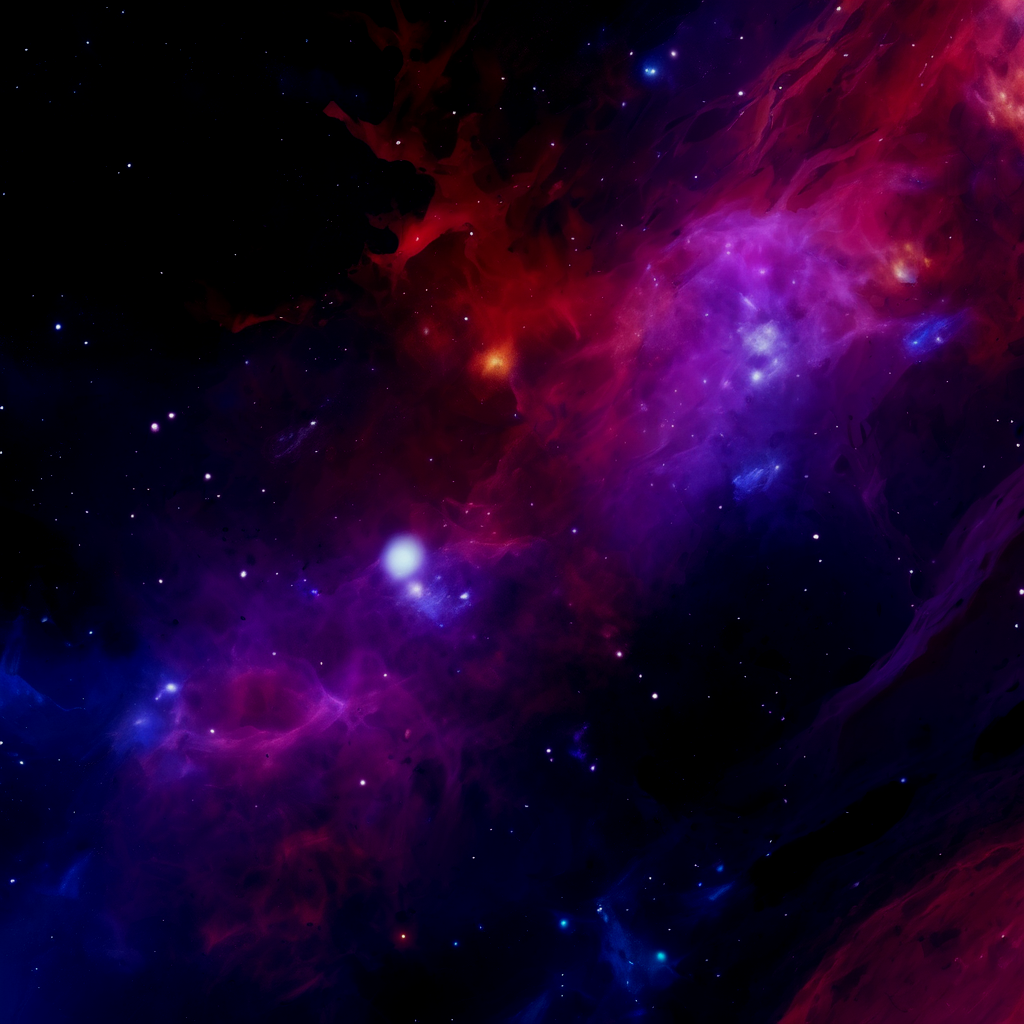
\includegraphics[height=\paperheight,width=\paperwidth]{fondo}};
  \end{tikzpicture}
}%
\usetikzlibrary{arrows.meta, decorations.pathmorphing,positioning,trees}

\lstset{
    basicstyle=\ttfamily\small,
    breaklines=true,
    backgroundcolor=\color{black!98},
    keywordstyle=\color{Magenta},
    commentstyle=\color{AntiqueWhite},
    stringstyle=\color{Yellow!80!white},
    showstringspaces=false,
    frame=single,
    rulecolor=\color{mypurple},
    frameround=tttt,
    escapeinside={\%*}{*)}
}

\makeatletter
% Set victor mono as default ttfont
\newtcolorbox{blur}[1][]{%
  #1,
  enhanced,
  remember,
  breakable, % Already enabled (good!)
  frame hidden,
  interior hidden,
  fonttitle=\bfseries\centering, 
  fontupper=\rmfamily\selectfont,
  coltext=white,
  underlay={
    \begin{tcbclipframe}
      \begin{scope}[inner sep=0pt,remember picture,overlay]
        \fill[white] (frame.south west) rectangle (frame.north east); % Changed to `frame` (not `current page`)
        \node[opacity=1] at (frame.center) {
\includegraphics[height=\paperheight, width=\paperwidth]{blured}};
      \end{scope}
    \end{tcbclipframe}
  }
}
\makeatother
%%%%%%%%%%%%%%%%%%%%%%%%%%%%%%%%%%%%%%%%%%%%%%%%%%%%%%%%%%%%%%%%%%%%%%%%
\newcommand{\separador}[1]{
  \vskip-4pt
  \begin{center}
    \rule{0.9\linewidth}{#1}
  \end{center}
}

\lstset{
  basicstyle=\ttfamily,
  showstringspaces=false,
  breaklines=true
}

\newcommand{\transparencia}[1]{%
  \begin{frame}
    \begin{blur}
      #1
    \end{blur}
  \end{frame}
}

% set bibliography background for text to be legible despite the background

\usepackage{etoolbox}
\newcommand{\setupblurbibliography}{%
  \pretocmd{\frametitle}{\blurbackground}{}{}%
  \setbeamertemplate{bibliography item}{\color{LimeGreen!80!White}\insertbiblabel}%
  \setbeamercolor{bibliography entry author}{fg=AntiqueWhite}%
  \setbeamercolor{bibliography entry title}{fg=Yellow!80!White}%
  \setbeamercolor{bibliography entry location}{fg=AntiqueWhite}%
  \setbeamercolor{bibliography entry note}{fg=AntiqueWhite}%
  \setbeamercolor{bibliography entry url}{fg=Magenta}%
}

\newtcblisting{beamerlst}[1][]{
    enhanced,
    breakable,
    listing only,
    listing options={
        style=beamerlisting,
        language=Python, % Default language
        #1
    },
    colback=black!85, % Matches your theme
    colframe=mypurple, % Your purple color
    fontupper=\ttfamily\small,
    arc=3mm, % Rounded corners
    boxrule=1pt,
    % Blur effect (optional):
    underlay={
        \begin{tcbclipframe}
        \fill[black!90] (frame.south west) rectangle (frame.north east);
        \node[opacity=0.6] at (frame.center) 
            {
\includegraphics[width=\linewidth]{blured}};
        \end{tcbclipframe}
    }
}

% Supporting style definition
\lstdefinestyle{beamerlisting}{
    basicstyle=\ttfamily\footnotesize\color{white},
    keywordstyle=\color{Magenta},
    commentstyle=\color{AntiqueWhite},
    stringstyle=\color{Yellow!80!white},
    showstringspaces=false,
    breaklines=true,
    tabsize=2
}

\newcommand{\codebox}[2][]{%
    \begin{tcolorbox}[
        enhanced,
        colback=black!85,
        colframe=mypurple,
        arc=3mm,
        boxrule=1pt,
        #1
    ]
    \lstinputlisting{#2}
    \end{tcolorbox}%
}

% Smart blur background that works with frame breaks
\newcommand{\blurbackground}{%
  \begin{tikzpicture}[remember picture,overlay]
    % Calculate content area with margins
    \path ([xshift=1cm,yshift=-1cm]current page.north west) coordinate (top left);
    \path ([xshift=-1cm,yshift=1cm]current page.south east) coordinate (bottom right);
    
    % Frosted glass effect
    \fill[black!85,opacity=0.92] (top left) rectangle (bottom right);
    \node[opacity=0.8] at (current page.center) 
      {
\includegraphics[width=\paperwidth-2cm,height=\paperheight-2cm]{blured}};
  \end{tikzpicture}%
}


\includeonly{01.-EvolutionaryComputing}

\bibliography{bibliografia}
\nocite{*}

\title{A Comparative Overview of Artificial Neural Network Architectures:
Theoretical Foundations and Applications}
\author{Brandon Marquez Salazar}

\begin{document}
\maketitle

\begin{abstract}

  Artificial Neural Network (ANN) architectures have rapidly diversified,
  each designed to address specific computational challenges and
  application domains. These architectures range from enhancements of
  foundational algorithms to specialized designs for particular
  problem-solving tasks. This overview examines prominent ANN
  architectures---including Feedforward Neural Networks (FFNs),
  Convolutional Neural Networks (CNNs), Recurrent Neural Networks (RNNs),
  Transformers, and Generative Models---and their applications in fields
  such as geotechnical engineering, energy forecasting, and computer
  vision. Based on a meta-analysis of recent literature, this review
  highlights key architectural innovations, provides performance
  comparisons, and discusses emerging trends within the field.

\end{abstract}

\section{Introduction}
\label{sec:introduction}

 The field of Artificial Intelligence (AI) was mainly fueled
 by the development of Artificial Neural Networks (ANNs). Inspired by
 biological neural research in attempts of understanding the neuronal
 behaviour. ANNs are computational models capable of
 learning complex, non-linear patterns from data \cite{lecun2015deep}.
 Over time, a diverse ecosystem of architectures has emerged, each
 designed to address specific computational challenges.

 From the foundational Feedforward Neural Networks (FFNs)
 \cite{rumelhart1986learning} to the specialized designs of Convolutional
 Neural Networks (CNNs) \cite{he2016deep} for spatial data and Recurrent
 Neural Networks (RNNs) \cite{hochreiter1997long} for time series, the
 evolution of ANNs has been driven by the need of reaching enhanced performance,
 better efficiency and extended applicability. More recently, the Transformer
 architecture \cite{vaswani2017attention} has revolutionized natural
 language processing and is now challenging CNNs in computer vision
 \cite{dosovitskiy2020image}. Simultaneously, Generative Models like GANs
 \cite{goodfellow2014generative} and VAEs \cite{kingma2013auto} have
 opened new frontiers in creating novel, realistic data.

 This review provides a structured overview of these key ANN
 architectures, focusing on their theoretical underpinnings, architectural
 innovations, and performance characteristics. Based on a meta-analysis of
 recent literature, this paper aims to synthesize the strengths and
 limitations of each paradigm and highlight emerging trends that are
 shaping the future of deep learning. The review is structured according
 to the IMRaD format, covering the core methodologies (architectures),
 results (performance comparisons), and discussion (trends and
 conclusions).

\section{Architectural Overview}
\label{sec:methods}

 This section delineates the fundamental architectures under review,
 detailing their core structural principles and theoretical innovations.

\subsection{Feedforward Neural Networks (FFNs)}

 FFNs, or Multi-Layer Perceptrons (MLPs), represent the simplest class of
 ANNs. They consist of an input layer, one or more hidden layers, and an
 output layer, with information flowing strictly forward without cycles.
 Their training is enabled by the backpropagation algorithm
 \cite{rumelhart1986learning}, which calculates the gradient of the loss
 function with respect to each weight. Theoretically, FFNs are universal
 function approximators but lack internal memory, making them suitable for
 static pattern recognition but ineffective for sequential data.

\subsection{Convolutional Neural Networks (CNNs)}

 CNNs are the dominant architecture for processing grid-like data such as
 images. Their design incorporates three key ideas to exploit spatial
 locality: (1) \textit{sparse connectivity} (neurons connect only to local
 regions), (2) \textit{parameter sharing} (using the same weights across
 spatial locations), and (3) \textit{hierarchical feature learning}
 \cite{lecun2015deep}. Architectures like ResNet \cite{he2016deep}
 introduced skip connections to mitigate the vanishing gradient problem in
 very deep networks, while designs like Xception
 \cite{chollet2017xception} further improved parameter efficiency through
 depthwise separable convolutions.

\ subsection{Recurrent Neural Networks (RNNs)}

 RNNs are designed for sequential data by introducing cyclic connections,
 allowing them to maintain an internal state or "memory" of previous
 inputs. The Long Short-Term Memory (LSTM) unit \cite{hochreiter1997long}
 was a pivotal innovation, introducing gating mechanisms (input, forget,
 and output gates) to regulate information flow and effectively learn
 long-range dependencies, overcoming the vanishing gradient problem of
 vanilla RNNs.

\subsection{Transformer Networks}

 The Transformer architecture \cite{vaswani2017attention} marked
 a paradigm shift by abandoning recurrence and convolution entirely. Its
 core mechanism is \textit{self-attention}, which weighs the significance
 of all elements in a sequence simultaneously when processing any single
 element. This allows for direct modeling of long-range dependencies and
 massive parallelization during training. The Vision Transformer (ViT)
 \cite{dosovitskiy2020image} demonstrated that this architecture could be
 applied directly to sequences of image patches, achieving
 state-of-the-art results in classification.

\subsection{Generative Models}

 This class of models learns the underlying probability distribution of
 data to generate novel samples. 

\begin{itemize}

   \item \textbf{Generative Adversarial Networks (GANs)}
       \cite{goodfellow2014generative} frame learning as an adversarial game
       between a generator (that creates fake data) and a discriminator
       (that distinguishes real from fake).

   \item \textbf{Variational Autoencoders (VAEs)} \cite{kingma2013auto}
       take a probabilistic approach, learning a latent representation of
       the data and generating new data by sampling from this latent space.

\end{itemize}

\section{Performance and Applications}
\label{sec:results}

 The efficacy of each architecture is contingent on its alignment with the
 problem domain. This section synthesizes their performance across key
 applications.

\subsection{Computer Vision}

 In image classification, CNNs like ResNet \cite{he2016deep} have long
 been the benchmark due to their efficient spatial feature extraction.
 However, Vision Transformers (ViTs) \cite{dosovitskiy2020image} have
 demonstrated comparable or superior performance on large datasets,
 leveraging their ability to model global context. For dense prediction
 tasks like image segmentation, Fully Convolutional Networks (FCNs) and
 specifically the U-Net architecture \cite{ronneberger2015u}—with its
 encoder-decoder structure and skip connections—remain the gold standard,
 effectively combining high-level semantics with low-level spatial
 precision.

\subsection{Sequential and Temporal Data}

 RNNs and their LSTM variants \cite{hochreiter1997long} have been widely
 successful in time-series forecasting and natural language processing due
 to their inherent temporal dynamics. The Transformer
 \cite{vaswani2017attention} has largely superseded them in NLP by
 offering superior training speed and performance on large datasets,
 thanks to parallelization and global context awareness. Hybrid models,
 such as the Meta-ANN for Short-Term Load Forecasting \cite{Xiao2022},
 showcase how dynamic architectures refined by meta-learning can
 outperform static models by adapting to non-stationary patterns.

\subsection{Generative Tasks}

 GANs \cite{goodfellow2014generative} are renowned for generating
 high-fidelity, sharp images, though their training can be unstable and
 prone to mode collapse. VAEs \cite{kingma2013auto}, in contrast, provide
 a more stable training process and a structured latent space but often
 produce blurrier samples. The choice between them involves a trade-off
 between sample quality and training stability.

\section{Discussion}
\label{sec:discussion}

 The evolution of ANN architectures reveals a clear trend: from
 general-purpose function approximators to highly specialized designs, and
 now towards a new synthesis of these specializations. The comparative
 analysis indicates that there is no single "best" architecture; rather,
 the optimal choice is dictated by the inductive biases required for the
 task—spatial invariance for images, temporal consistency for sequences,
 and the ability to model data distributions for generation.

 A key emerging trend is the \textit{hybridization} of architectural
 paradigms. The Vision Transformer is a prime example, applying
 a sequence-modeling architecture to computer vision
 \cite{dosovitskiy2020image}. Similarly, models like Meta-ANN
 \cite{Xiao2022} integrate meta-learning to create dynamic networks that
 adapt to changing data distributions, pointing towards more robust and
 generalizable systems.

 Future research directions are likely to focus on several areas: (1)
 improving the computational and energy efficiency of large models like
 Transformers, (2) enhancing the stability and controllability of
 generative models, and (3) automating architecture design through Neural
 Architecture Search (NAS). Furthermore, the development of architectures
 that can seamlessly learn from multiple data modalities (vision,
 language, sound) within a single model represents a significant frontier
 in AI research.

\printbibliography
\end{document}
